\chapter{Specifikacija programske potpore}
		
	\section{Funkcionalni zahtjevi}
			
			%\textbf{\textit{dio 1. revizije}}\\
			
			%\textit{Navesti \textbf{dionike} koji imaju \textbf{interes u ovom sustavu} ili  \textbf{su nositelji odgovornosti}. To su prije svega korisnici, ali i administratori sustava, naručitelji, razvojni tim.}\\
				
		%	\textit{Navesti \textbf{aktore} koji izravno \textbf{koriste} ili \textbf{komuniciraju sa sustavom}. Oni mogu imati inicijatorsku ulogu, tj. započinju određene procese u sustavu ili samo sudioničku ulogu, tj. obavljaju određeni posao. Za svakog aktora navesti funkcionalne zahtjeve koji se na njega odnose.}\\
			
			
			\noindent \textbf{Dionici:}
			
			\begin{packed_enum}
				
				\item Vlasnik (naručitelj)
				\item Klijenti
				\begin{packed_enum}
					\item Privatni
					\item Poslovni
				\end{packed_enum}				
				\item Administrator
				\item Razvojni tim
				
			\end{packed_enum}
			
			\noindent \textbf{Aktori i njihovi funkcionalni zahtjevi:}
			
			
			\begin{packed_enum}
				\item  \underbar{Neregistrirani/neprijavljeni korisnik (inicijator) može:}
				
				\begin{packed_enum}
					
					\item jednostavno mijenjati  kontekst  iz  privatnog  u  poslovni  i  obrnuto
					\item pregledavati predefinirane izbore boja, vrsta, težina i formata papira
				%	\begin{packed_enum}
						
					%	\item  podfunkcionalnost 1 
					%	\item  podfunkcionalnost 2
				
				%	\end{packed_enum}
				%	\item  funkcionalnost 3
					
				\end{packed_enum}
			
				\item  \underbar{Privatni klijent (inicijator) može:}
				
				\begin{packed_enum}
					
					\item odabrati predefinirane izbore boja, vrsta, težina i formata papira i platiti svoju narudžbu
					
				\end{packed_enum}
			
				\item  \underbar{Poslovni klijent (inicijator) može:}
				
				\begin{packed_enum}
					
					\item odabrati predefinirane izbore boja, vrsta, težina i formata papira i platiti svoju narudžbu
					
					\item odabrati papir nekonvencionalnih veličina i dodati vodeni žig
					
					\item zatražiti dodatne usluge koje nisu na ponudi
					
					\item  pregledavati i odabrati potvrđene dodatne usluge
					
					\item zakazati, pregledavati i otkazivati mjesečne pretplate
					
				\end{packed_enum}
			
				\item  \underbar{Administrator (inicijator) može:}
				
				\begin{packed_enum}
					
					\item pregledavanti pojedine tekstualne zahtjeve poslovnih klijenata, te potvrditi ili odbiti i uklanjati iste
					
					\item pregledavati i otkazivati mjesečne pretplate
					
					\item pregledavati povijest kupljenih usluga za  sve  korisnike
					
				\end{packed_enum}
				
				\item  \underbar{Baza podataka (sudionik) može:}
				
				\begin{packed_enum}
					
					\item pohranjivati podatke o klijentima
					\item pohranjivati podatke o artiklima na ponudi
					\item pohranjivati narudžbe
					
				\end{packed_enum}
			\end{packed_enum}
			
			\eject 
			
			
				
			\subsection{Obrasci uporabe}
				
				%\textbf{\textit{dio 1. revizije}}
				
				%\subsubsection{Opis obrazaca uporabe}
					%\textit{Funkcionalne zahtjeve razraditi u obliku obrazaca uporabe. Svaki obrazac je potrebno razraditi prema donjem predlošku. Ukoliko u nekom koraku može doći do odstupanja, potrebno je to odstupanje opisati i po mogućnosti ponuditi rješenje kojim bi se tijek obrasca vratio na osnovni tijek.}\\
					

					\noindent \underbar{\textbf{UC1-Pregled preddefiniranih papira}}
					\begin{packed_item}
	
						\item \textbf{Glavni sudionik: } Korisnik, klijent
						\item  \textbf{Cilj:} Pregledavanje preddefiniranih artikala
						\item  \textbf{Sudionici:} Baza podataka
						\item  \textbf{Preduvjet:} -
						\item  \textbf{Opis osnovnog tijeka:}
						
						\item[] \begin{packed_enum}
	
							\item Korisnik odabire opciju za pregled papira u načinu za privatnog klijenta
							\item Korisnik pregledava postojeće opcije po padajućim izbornicima
						\end{packed_enum}
					
					\end{packed_item}
				
			
					\noindent \underbar{\textbf{UC2-Registracija privatnog klijenta}}
					\begin{packed_item}
						
						\item \textbf{Glavni sudionik: } Korisnik
						\item  \textbf{Cilj:} Stvoriti privatni korisnički račun
						\item  \textbf{Sudionici:} Baza podataka
						\item  \textbf{Preduvjet:} -
						\item  \textbf{Opis osnovnog tijeka:}
						
						\item[] \begin{packed_enum}
							
							\item Korisnik odabire opciju za registraciju privatnog klijenta
							\item Korisnik unosi potrebne korisničke podatke
							\item Korisnik prima obavijest o uspješnoj registraciji
						\end{packed_enum}
						
						\item  \textbf{Opis mogućih odstupanja:}
						
						\item[] \begin{packed_item}
							
							\item[2.a]  Odabir već zauzetog korisničkog imena i/ili e-maila, unos korisničkog podatka u nedozvoljenom formatu ili pružanje neispravnoga e-maila
							\item[] \begin{packed_enum}
								
								\item Sustav obavještava korisnika o neuspjelom upisu i vraća ga na stranicu za registraciju
								\item  Korisnik mijenja potrebne podatke te završava unos ili odustaje od registracije
								
							\end{packed_enum}
						\end{packed_item}
					\end{packed_item}
				
					\noindent \underbar{\textbf{UC3-Registracija poslovnog klijenta}}
					\begin{packed_item}
						
						\item \textbf{Glavni sudionik: } Korisnik
						\item  \textbf{Cilj:} Stvoriti poslovni korisnički račun
						\item  \textbf{Sudionici:} Baza podataka
						\item  \textbf{Preduvjet:} -
						\item  \textbf{Opis osnovnog tijeka:}
						
						\item[] \begin{packed_enum}
							
							\item Korisnik odabire opciju za registraciju poslovnog klijenta
							\item Korisnik unosi potrebne korisničke podatke
							\item Korisnik prima obavijest o uspješnoj registraciji
						\end{packed_enum}
						
						\item  \textbf{Opis mogućih odstupanja:}
						
						\item[] \begin{packed_item}
							
							\item[2.a]  Odabir već zauzetog ili neispravnog imena kompanije, OIB-a, kontakt osobe, telefona i/ili e-maila
							\item[] \begin{packed_enum}
								
								\item Sustav obavještava korisnika o neuspjelom upisu i vraća ga na stranicu za registraciju
								\item  Korisnik mijenja potrebne podatke te završava unos ili odustaje od registracije
								
							\end{packed_enum}
						\end{packed_item}
					\end{packed_item}
				
					\noindent \underbar{\textbf{UC4-Prijava privatnog klijenta u sustav}}
					\begin{packed_item}
						
						\item \textbf{Glavni sudionik: } Privatni klijent
						\item  \textbf{Cilj:} Dobiti pristup korisničkom sučelju
						\item  \textbf{Sudionici:} Baza podataka
						\item  \textbf{Preduvjet:} Registracija
						\item  \textbf{Opis osnovnog tijeka:}
						
						\item[] \begin{packed_enum}
							
							\item Korisnik odabire opciju za registraciju privatnog klijenta
							\item Korisnik unosi potrebne korisničke podatke
							\item Korisnik prima obavijest o uspješnoj prijavi
							\item Korisnik gubi pristup poslovnim funkcijama
						\end{packed_enum}
						
						\item  \textbf{Opis mogućih odstupanja:}
						
						\item[] \begin{packed_item}
							
							\item[2.a]  Neispravno ime i/ili lozinka
							\item[] \begin{packed_enum}
								
								\item Sustav obavještava korisnika o neuspjelom upisu i vraća ga na stranicu za prijavu
								\item Korisnik ponovno unosi podatke za prijavu ili odustaje od prijave
							
							\end{packed_enum}
						\end{packed_item}
					\end{packed_item}
				
					\noindent \underbar{\textbf{UC5-Prijava poslovnog klijenta u sustav}}
					\begin{packed_item}
						
						\item \textbf{Glavni sudionik: } Poslovni klijent
						\item  \textbf{Cilj:} Dobiti pristup korisničkom sučelju
						\item  \textbf{Sudionici:} Baza podataka
						\item  \textbf{Preduvjet:} Registracija
						\item  \textbf{Opis osnovnog tijeka:}
						
						\item[] \begin{packed_enum}
							
							\item Korisnik odabire opciju za registraciju poslovnog klijenta
							\item Korisnik unosi potrebne korisničke podatke
							\item Korisnik prima obavijest o uspješnoj prijavi
						\end{packed_enum}
						
						\item  \textbf{Opis mogućih odstupanja:}
						
						\item[] \begin{packed_item}
							
							\item[2.a]  Neispravno ime i/ili lozinka
							\item[] \begin{packed_enum}
								
								\item Sustav obavještava korisnika o neuspjelom upisu i vraća ga na stranicu za prijavu
								\item Korisnik ponovno unosi podatke za prijavu ili odustaje od prijave
								
							\end{packed_enum}
						\end{packed_item}
					\end{packed_item}
				
					\noindent \underbar{\textbf{UC6-Dodavanje usluge u košaricu}}
					\begin{packed_item}
						
						\item \textbf{Glavni sudionik: } Klijent
						\item  \textbf{Cilj:} Dodati uslugu u košaricu
						\item  \textbf{Sudionici:} -
						\item  \textbf{Preduvjet:} Korisnik je prijavljen
						\item  \textbf{Opis osnovnog tijeka:}
						
						\item[] \begin{packed_enum}
							
							\item Klijent odabire preddefiniranu uslugu
							\item Klijent odabire opciju "Dodaj u košaricu"
						\end{packed_enum}
					
						\item  \textbf{Opis mogućih odstupanja:}
						
						\item[] \begin{packed_item}
							
							\item[2.a]  Nisu odabrani svi podaci o papiru
							\item[] \begin{packed_enum}
								
								\item Sustav obavještava klijenta o neuspjelom odabiru i pita ga da provjeri podatke
								\item  Klijent odabire potrebne podatke te odabire opciju "Dodaj u košaricu" ili odustaje od dodavanja
							\end{packed_enum}
						\end{packed_item}
					\end{packed_item}
				
					\noindent \underbar{\textbf{UC7-Dodavanje papira posebne dimenzije i/ili sa žigom u košaricu}}
					\begin{packed_item}
						
						\item \textbf{Glavni sudionik: } Poslovni klijent
						\item  \textbf{Cilj:} Dodati papira posebne dimenzije i/ili sa žigom u košaricu
						\item  \textbf{Sudionici:} -
						\item  \textbf{Preduvjet:} Korisnik je prijavljen
						\item  \textbf{Opis osnovnog tijeka:}
						
						\item[] \begin{packed_enum}
							
							\item Klijent odabire dimenzije papira i/ili priloži sliku vodenog žiga
							\item Klijent odabire opciju "Dodaj u košaricu"
						\end{packed_enum}
						
						\item  \textbf{Opis mogućih odstupanja:}
						
						\item[] \begin{packed_item}
							
							\item[2.a]  Dimenzije izvan određenih granica ili u krivom formatu
							\item[] \begin{packed_enum}
								
								\item Sustav obavještava klijenta o neuspjelom upisu i pita ga da provjeri podatke
								\item  Klijent mijenja potrebne podatke te odabire opciju "Dodaj u košaricu" ili odustaje od dodavanja
								
							\end{packed_enum}
						
							\item[2.b]  Vodeni žig u krivom formatu
							\item[] \begin{packed_enum}
								\item Sustav obavještava klijenta o neuspjelom prilogu žiga i obavještava ga da je potrebna slika žiga
								\item klijent prilaže sliku te odabire opciju "Dodaj u košaricu" ili odustaje od dodavanja
						\end{packed_enum}
					\end{packed_item}
				\end{packed_item}
				
				\noindent \underbar{\textbf{UC8-Slanje tekstualnog zahtjeva za dodatne usluge}}
				\begin{packed_item}
					
					\item \textbf{Glavni sudionik: } Poslovni klijent
					\item  \textbf{Cilj:}  Zatražiti uslugu koja nije na ponudi
					\item  \textbf{Sudionici:} Baza podataka, administrator
					\item  \textbf{Preduvjet:} Korisnik je prijavljen
					\item  \textbf{Opis osnovnog tijeka:}
					
					\item[] \begin{packed_enum}
						
						\item Klijent odabire opciju za slanje tekstualnog zahtjeva
						\item Klijent unosi zahtjev, naziv usluge i kontakt podatke
						\item Klijent prima obavijest da njegov zahtjev čeka potvrdu
					
					\end{packed_enum}
					
					\item  \textbf{Opis mogućih odstupanja:}
					
					\item[] \begin{packed_item}
						
						\item[2.a]  Unesen zahtjev i opis su prazni
						\item[] \begin{packed_enum}
							
							\item Sustav obavještava klijenta da zahtjevi ne mogu biti prazni
							\item  Klijent unosi potrebne podatke te završava unos ili odustaje od zahtjeva
							
						\end{packed_enum}
					
						\item[2.b]  Uneseni neispravni kontakt podaci
						\item[] \begin{packed_enum}
							
							\item Sustav obavještava klijenta o neispravnosti kontakt podataka
							\item  Klijent mijenja kontakt podatke te završava unos ili odustaje od registracije
							
						\end{packed_enum}
					\end{packed_item}
				\end{packed_item}
			
				\noindent \underbar{\textbf{UC9-Zakazivanje mjesečne pretplate}}
				\begin{packed_item}
					
					\item \textbf{Glavni sudionik: } Poslovni klijent
					\item  \textbf{Cilj:} Zakazivanje mjesečne pretplate za pojedine usluge
					\item  \textbf{Sudionici:} Baza podataka
					\item  \textbf{Preduvjet:} Korisnik je prijavljen
					\item  \textbf{Opis osnovnog tijeka:}
					
					\item[] \begin{packed_enum}
						
						\item Klijent odabire svoju košaricu
						\item Klijent u košarici odabire usluge za koje želi mjesečnu pretplatu i označava ih
					
					\end{packed_enum}
					
				\end{packed_item}
			
				\noindent \underbar{\textbf{UC10-Pregled mjesečnih pretplata}}
				\begin{packed_item}
					
					\item \textbf{Glavni sudionik: } Poslovni klijent
					\item  \textbf{Cilj:} Pregledavanje aktivnih mjesečnih pretplata
					\item  \textbf{Sudionici:} Baza podataka
					\item  \textbf{Preduvjet:} Korisnik je prijavljen
					\item  \textbf{Opis osnovnog tijeka:}
					
					\item[] \begin{packed_enum}
						
						\item Klijent odabire opciju za pregled mjesečnih pretplata
						
					\end{packed_enum}
					
				\end{packed_item}
			
				\noindent \underbar{\textbf{UC11-Otkazivanje mjesečnih pretplata}}
				\begin{packed_item}
					
					\item \textbf{Glavni sudionik: } Poslovni klijent
					\item  \textbf{Cilj:} Otkazivanje mjesečnih pretplata
					\item  \textbf{Sudionici:} Baza podataka, administrator
					\item  \textbf{Preduvjet:} Korisnik je prijavljen i postoje mjesečne pretplate
					\item  \textbf{Opis osnovnog tijeka:}
					
					\item[] \begin{packed_enum}
						
						\item Klijent odabire opciju za pregled mjesečnih pretplata
						\item Klijent odabire mjesečnu pretplatu koju želi otkazati
						\item Klijent prima obavijest da je pretplata otkazana
						
					\end{packed_enum}
					
				\end{packed_item}
			
				\noindent \underbar{\textbf{UC12-Pregled sadržaja košarice}}
				\begin{packed_item}
					
					\item \textbf{Glavni sudionik: } Klijent
					\item  \textbf{Cilj:} Prikaz i pregled sadržaja košarice
					\item  \textbf{Sudionici:} -
					\item  \textbf{Preduvjet:} Korisnik je prijavljen
					\item  \textbf{Opis osnovnog tijeka:}
					
					\item[] \begin{packed_enum}
						
						\item Klijent odabire opciju za pregled košarice
						
					\end{packed_enum}
					
				\end{packed_item}
			
				\noindent \underbar{\textbf{UC13-Uređivanje sadržaja košarice}}
				\begin{packed_item}
					
					\item \textbf{Glavni sudionik: } Klijent
					\item  \textbf{Cilj:} Micanje usluga iz košarice, promjena kvantitete
					\item  \textbf{Sudionici:} -
					\item  \textbf{Preduvjet:} Korisnik je prijavljen
					\item  \textbf{Opis osnovnog tijeka:}
					
					\item[] \begin{packed_enum}
						
						\item Klijent odabire opciju za pregled košarice
						\item Klijent makne i/ili uređuje usluge u košarici
						
					\end{packed_enum}
				
				\end{packed_item}
			
				\noindent \underbar{\textbf{UC14-Naručivanje usluga}}
				\begin{packed_item}
					
					\item \textbf{Glavni sudionik: } Klijent
					\item  \textbf{Cilj:} Potvrditi narudžbu kako bi ju mogao platiti
					\item  \textbf{Sudionici:} -
					\item  \textbf{Preduvjet:} Korisnik je prijavljen
					\item  \textbf{Opis osnovnog tijeka:}
					
					\item[] \begin{packed_enum}
						
						\item Klijent odabire opciju za pregled košarice
						\item Klijent odabire opciju za naručivanje
						\item Klijent se usmjeri na plaćanje usluge
						
					\end{packed_enum}
					
					\item  \textbf{Opis mogućih odstupanja:}
					
					\item[] \begin{packed_item}
						
						\item[2.a] Košarica je prazna
						\item[] \begin{packed_enum}
							
							\item Klijenta sustav obavijesti da se narudžba provodi samo nad nepraznom košaricom i vraća ga se na pregled košarice
							
						\end{packed_enum}
						
					\end{packed_item}
				\end{packed_item}
			
				\noindent \underbar{\textbf{UC15-Plaćanje usluge}}
				\begin{packed_item}
					
					\item \textbf{Glavni sudionik: } Klijent
					\item  \textbf{Cilj:} Plaćanje usluge kako bi proces kupnje usluge bio završen
					\item  \textbf{Sudionici:} Baza podataka
					\item  \textbf{Preduvjet:} Korisnik je prijavljen
					\item  \textbf{Opis osnovnog tijeka:}
					
					\item[] \begin{packed_enum}
						
						\item Klijent za odabranu opciju plaćanja unosi svoje podatke
						\item Klijent potvrđuje plaćanje
						\item Košarica se isprazni i klijenta se vraća na pregled košarice
					\end{packed_enum}
					
					\item  \textbf{Opis mogućih odstupanja:}
					
					\item[] \begin{packed_item}
						
						\item[2.a] Nedovoljan iznos na računu za plaćanje narudžbe
						\item[] \begin{packed_enum}
							
							\item Klijenta se obavještava da je iznos nedostatan za plaćanje narudžbe i vraća ga na pregled košarice
							
						\end{packed_enum}
						
					\end{packed_item}
				\end{packed_item}
			
				\noindent \underbar{\textbf{UC16-Prikaz povijesti kupljenih usluga za sve korisnike}}
				\begin{packed_item}
					
					\item \textbf{Glavni sudionik: } Administrator
					\item  \textbf{Cilj:} Prikaz povijesti kupljenih usluga za sve korisnike
					\item  \textbf{Sudionici:} Baza podataka
					\item  \textbf{Preduvjet:} Korisnik je prijavljen
					\item  \textbf{Opis osnovnog tijeka:}
					
					\item[] \begin{packed_enum}
						
						\item Administrator odabire opciju za prikaz povijesti kupljenih usluga
					\end{packed_enum}
					
				\end{packed_item}

				\noindent \underbar{\textbf{UC17-Prikaz vlastite povijesti kupljenih usluga}}
				\begin{packed_item}
					
					\item \textbf{Glavni sudionik: } Klijent
					\item  \textbf{Cilj:} Prikaz vlastite povijesti kupljenih usluga
					\item  \textbf{Sudionici:} Baza podataka
					\item  \textbf{Preduvjet:} Korisnik je prijavljen
					\item  \textbf{Opis osnovnog tijeka:}
					
					\item[] \begin{packed_enum}
						
						\item Klijent odabire opciju za prikaz povijesti kupljenih usluga
						
					\end{packed_enum}
				\end{packed_item}
			
				\noindent \underbar{\textbf{UC18-Potvrđivanje dodatnih usluga}}
				\begin{packed_item}
					
					\item \textbf{Glavni sudionik: } Administrator, poslovni klijent
					\item  \textbf{Cilj:} Potvrđivanje i dodavanje dodatnih usluga, poslanih tekstualnim zahtjevom, poslovnom klijentu
					\item  \textbf{Sudionici:} Baza podataka
					\item  \textbf{Preduvjet:} Administrator je prijavljen i tekstualni zahtjev postoji
					\item  \textbf{Opis osnovnog tijeka:}
					
					\item[] \begin{packed_enum}
						
						\item Administrator odabire opciju za prikaz tekstualnih zahtjeva koji čekaju potvrdu
						\item Administrator odabire zahtjev koji želi potvrditi i potvrđuje ga
						\item Zahtjev se makne iz administratorovog prikaza tekstualnih zahtjeva koji čekaju potvrdu i prikazuje u opciji dodatnih usluga poslovnog klijenta čiji je zahtjev potvrđen
						
					\end{packed_enum}
					
				%	\item  \textbf{Opis mogućih odstupanja:}
					
				%	\item[] \begin{packed_item}
						
					%	\item[2.a] $<$opis mogućeg scenarija odstupanja u koraku 2$>$
					%	\item[] \begin{packed_enum}
							
						%	\item $<$opis rješenja mogućeg scenarija korak 1$>$
						%	\item $<$opis rješenja mogućeg scenarija korak 2$>$
							
						%\end{packed_enum}
						%\item[2.b] $<$opis mogućeg scenarija odstupanja u koraku 2$>$
					%	\item[3.a] $<$opis mogućeg scenarija odstupanja  u koraku 3$>$
						
				%	\end{packed_item}
				\end{packed_item}
			
				\noindent \underbar{\textbf{UC19-Odbijanje dodatnih usluga}}
				\begin{packed_item}
					
					\item \textbf{Glavni sudionik: } Administrator, poslovni klijent
					\item  \textbf{Cilj:} Odbijanje dodatnih usluga, poslanih tekstualnim zahtjevom, poslovnom klijentu
					\item  \textbf{Sudionici:} Baza podataka
					\item  \textbf{Preduvjet:} Administrator je prijavljen i tekstualni zahtjev postoji
					\item  \textbf{Opis osnovnog tijeka:}
					
					\item[] \begin{packed_enum}
						
						\item Administrator odabire opciju za prikaz tekstualnih zahtjeva koji čekaju potvrdu
						\item Administrator odabire zahtjev koji želi odbiti i odbija ga
						\item Zahtjev se makne iz administratorovog prikaza tekstualnih zahtjeva koji čekaju potvrdu i obavještava se poslovnog klijenta kojem je zahtjev odbijen
						
					\end{packed_enum}
				\end{packed_item}
			
			
				\noindent \underbar{\textbf{UC20-Pregled potvrđenih dodatnih usluga}}
				\begin{packed_item}
					
					\item \textbf{Glavni sudionik: } Administrator
					\item  \textbf{Cilj:} Pregledavanje potvrđenih  dodatnih usluga
					\item  \textbf{Sudionici:} Baza podataka
					\item  \textbf{Preduvjet:} Administrator je prijavljen
					\item  \textbf{Opis osnovnog tijeka:}
					
					\item[] \begin{packed_enum}
						
						\item Administrator odabire opciju za pregled potvrđenih dodatnih usluga
						\item Administrator pregledava sve potvrđene dodatne usluge
						
					\end{packed_enum}
				\end{packed_item}
			
				
			
				\noindent \underbar{\textbf{UC21-Uklanjanje potvrđenih dodatnih usluga}}
				\begin{packed_item}
					
					\item \textbf{Glavni sudionik: } Administrator, poslovni klijent
					\item  \textbf{Cilj:} Uklanjanje potvrđenih dodatnih usluga iz ponude poslovnog klijenta
					\item  \textbf{Sudionici:} Baza podataka
					\item  \textbf{Preduvjet:} Administrator je prijavljen i potvrđene dodatne usluge postoje
					\item  \textbf{Opis osnovnog tijeka:}
					
					\item[] \begin{packed_enum}
						
						\item Administrator odabire opciju za prikaz potvrđenih dodatnih usluga
						\item Administrator odabire zahtjev koji želi ukloniti i uklanja ga
						\item Zahtjev se makne iz administratorovog prikaza potvrđenih dodatnih usluga, obavještava se poslovnog klijenta i uklanja mu se dodatna usluga kao i postojeće pretplate sa tom uslugom
						
					\end{packed_enum}
				\end{packed_item}
			
				\noindent \underbar{\textbf{UC22-Pregled dodatnih usluga}}
				\begin{packed_item}
					
					\item \textbf{Glavni sudionik: } Poslovni klijent
					\item  \textbf{Cilj:} Pregled dodatnih usluga ovog poslovnog klijenta
					\item  \textbf{Sudionici:} Baza podataka
					\item  \textbf{Preduvjet:} Korisnik je prijavljen
					\item  \textbf{Opis osnovnog tijeka:}
					
					\item[] \begin{packed_enum}
						
						\item Klijent odabire opciju za prikaz dodatnih usluga
						
					\end{packed_enum}
				\end{packed_item}

				\noindent \underbar{\textbf{UC23-Dodavanje dodatnih usluga u košaricu}}
				\begin{packed_item}
					
					\item \textbf{Glavni sudionik: } Poslovni klijent
					\item  \textbf{Cilj:} Dodavanje dodatnih usluga u košaricu
					\item  \textbf{Sudionici:} -
					\item  \textbf{Preduvjet:} Klijent je prijavljen
					\item  \textbf{Opis osnovnog tijeka:}
					
					\item[] \begin{packed_enum}
						
						\item Klijent odabire dodatnu uslugu među potvrđenim dodatnim uslugama i dodaje ju u košaricu 
						
						
					\end{packed_enum}
				
					
				
				
				\end{packed_item}
			
				\noindent \underbar{\textbf{UC24-Pregled mjesečnih pretplata poslovnih klijenata}}
				\begin{packed_item}
					
					\item \textbf{Glavni sudionik: } Administrator
					\item  \textbf{Cilj:} Pregledavanje aktivnih mjesečnih pretplata
					\item  \textbf{Sudionici:} Baza podataka
					\item  \textbf{Preduvjet:} Korisnik je prijavljen
					\item  \textbf{Opis osnovnog tijeka:}
					
					\item[] \begin{packed_enum}
						
						\item Administrator odabire pregled mjesečnih pretplata za poslovne korisnike
						
					\end{packed_enum}
					
				\end{packed_item}
			
				\noindent \underbar{\textbf{UC25-Otkazivanje mjesečne pretplate poslovnih klijenata}}
				\begin{packed_item}
					
					\item \textbf{Glavni sudionik: } Administrator
					\item  \textbf{Cilj:} Otkazivanje mjesečnih pretplata
					\item  \textbf{Sudionici:} Baza podataka
					\item  \textbf{Preduvjet:} Korisnik je prijavljen
					\item  \textbf{Opis osnovnog tijeka:}
					
					\item[] \begin{packed_enum}
						
						\item Administrator odabire pregled mjesečnih pretplata za poslovne korisnike
						\item Administrator otkazuje (deaktivira) odabranu mjesečnu pretplatu
						\item Administrator prima obavijest da je pretplata otkazana
						
					\end{packed_enum}
					
				\end{packed_item}
			
					
				\subsubsection{Dijagrami obrazaca uporabe}
					\begin{center}
						\begin{figure}[H]
							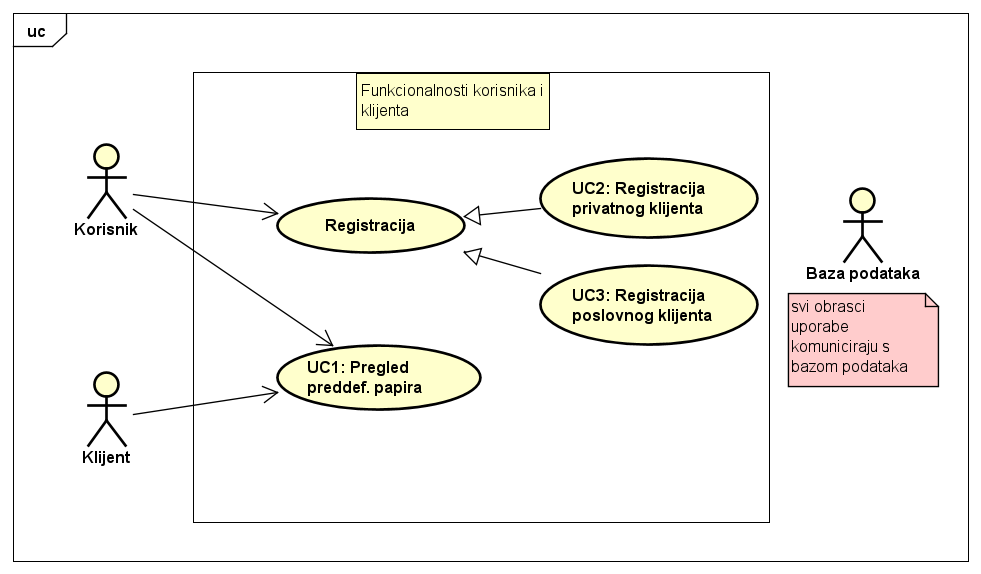
\includegraphics[scale=0.7]{dijagrami/korisnik_klijent.PNG} 
							\centering
							\caption{Dijagram obrazaca uporabe za korisnika i klijenta}
							\label{fig:obr_up1}%label mora biti drugaciji za svaku sliku
						\end{figure}
						
						\noindent \normalsize{   } \\
						\begin{figure}[H]
							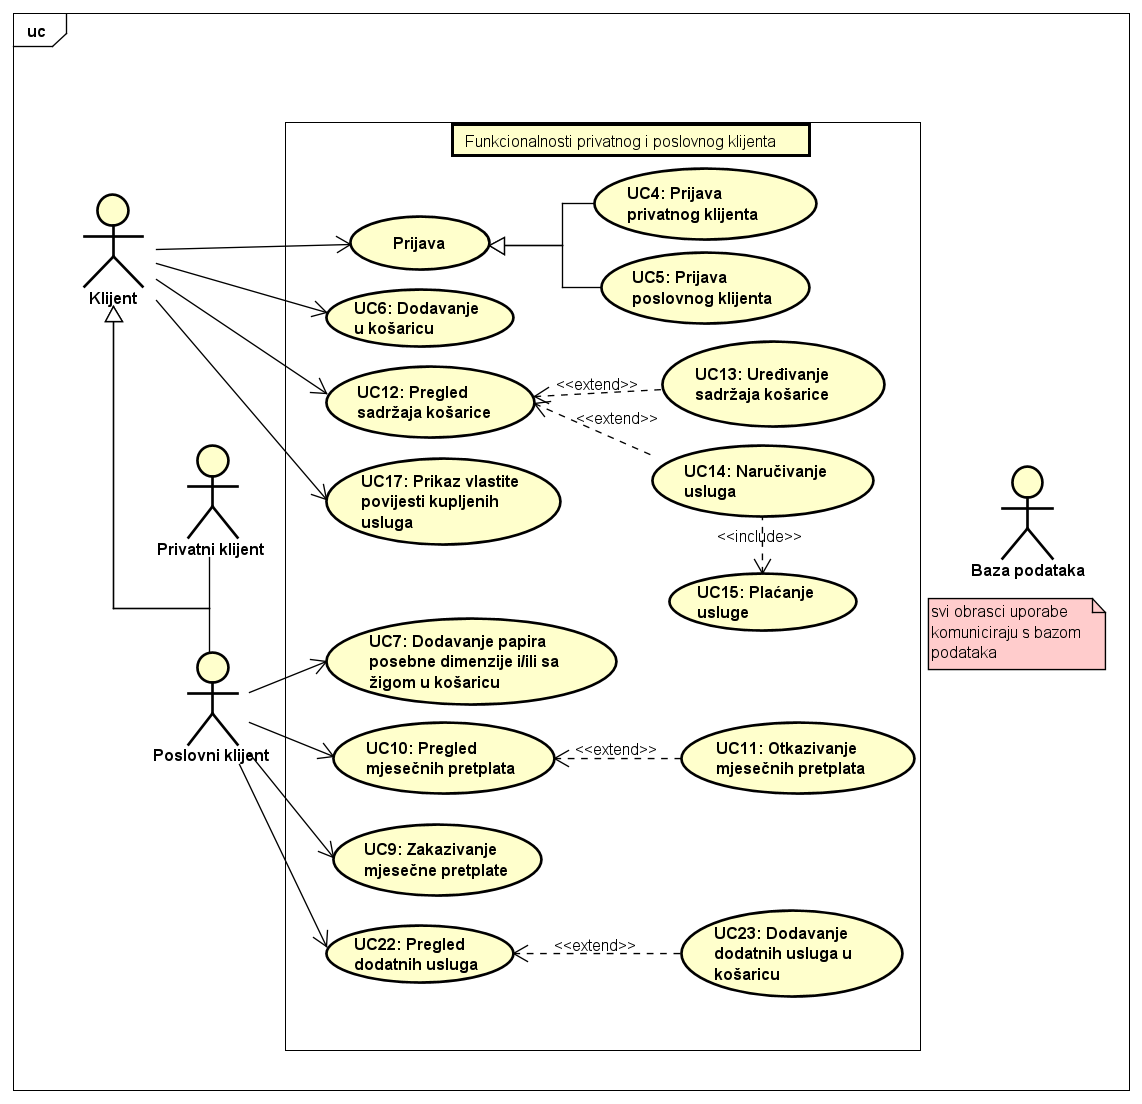
\includegraphics[scale=0.6]{dijagrami/privatni_poslovni.PNG} 
							\centering
							\caption{Dijagram obrazaca uporabe za privatne i poslovne klijente}
							\label{fig:obr_up2}%label mora biti drugaciji za svaku sliku
						\end{figure}
						\noindent \normalsize{   } \\
						\begin{figure}[H]
							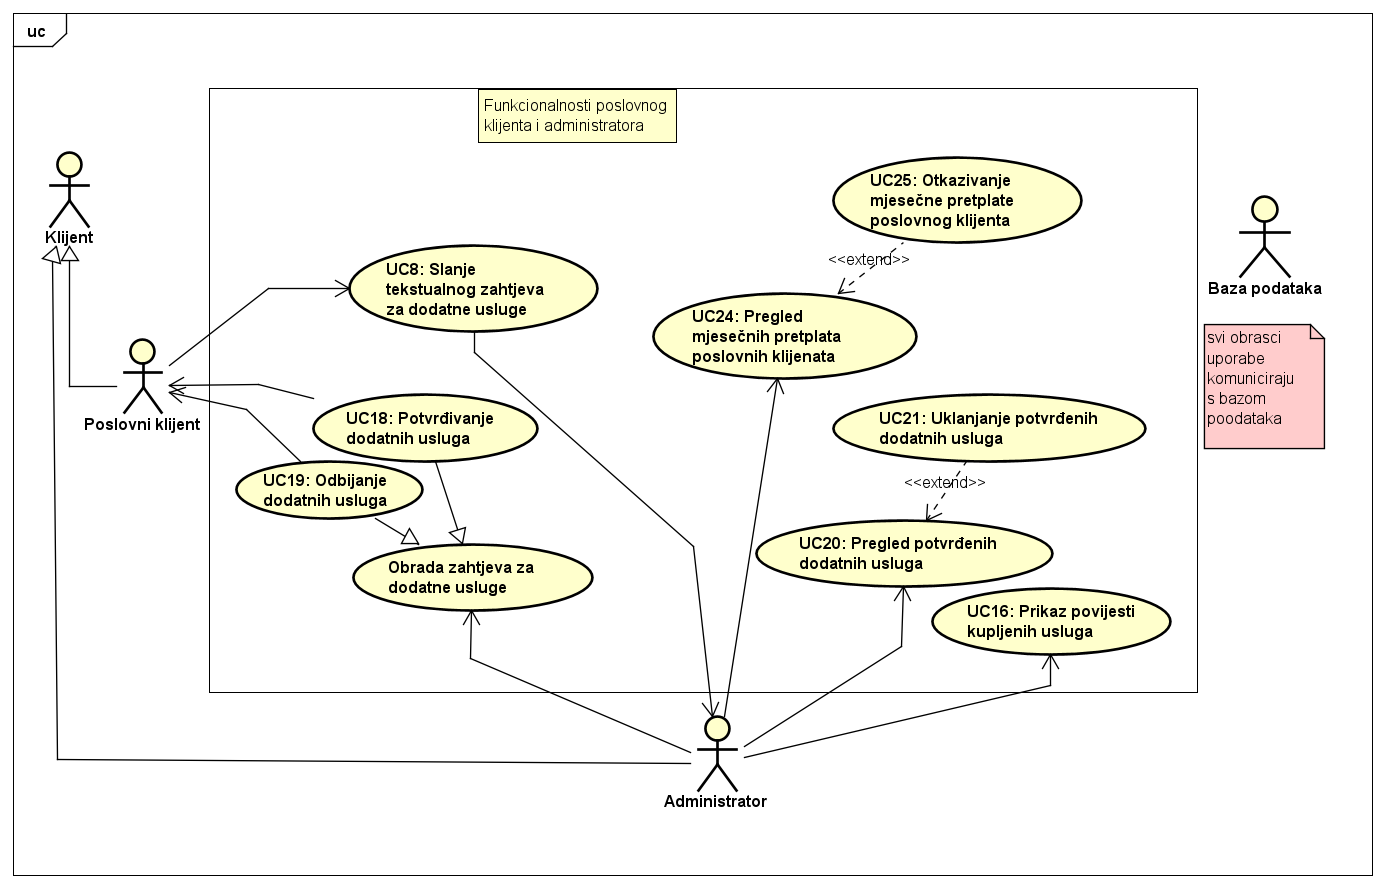
\includegraphics[scale=0.5]{dijagrami/poslovni_admin.PNG} 
							\centering
							\caption{Dijagram obrazaca uporabe za poslovne klijente i administratora}
							\label{fig:obr_up3}%label mora biti drugaciji za svaku sliku
						\end{figure}
						
					\end{center}
					
				\eject		
				
			\subsection{Sekvencijski dijagrami}
				
				\textbf{UC6: Dodavanje u košaricu}\\
				\noindent \normalsize{Klijent odabire parametre za željeni papir i stisne na gumb za dodavanje u košaricu. Ako su uneseni parametri ispravni (uneseni su svi i u pravilnom zapisu), onda se papir dodaje u košaricu. U suprotnom klijentu stiže poruka da nije odabrao sve parametre i košarica se ne mijenja.} \\
				\begin{figure}[H]
					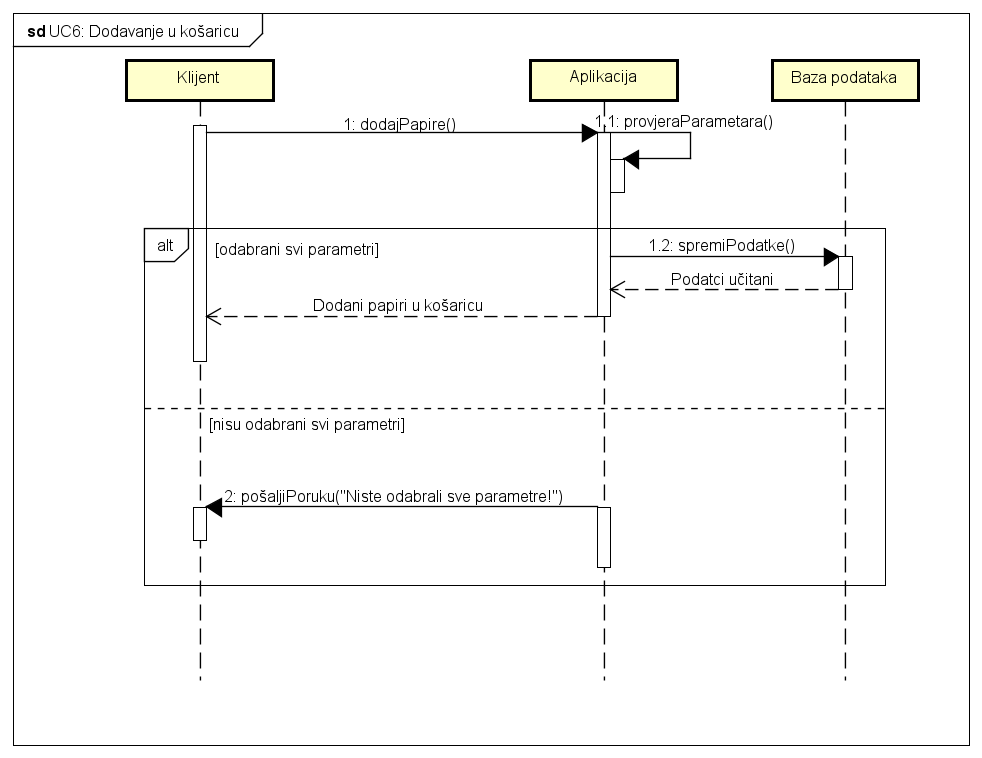
\includegraphics[scale=0.6]{dijagrami/sekv_uc6.PNG} 
					\centering
					\caption{Sekvencijski dijagram za UC6 - Dodavanje u košaricu}
					\label{fig:sekv_uc6}%label mora biti drugaciji za svaku sliku
				\end{figure}
			%	\textit{Nacrtati sekvencijske dijagrame koji modeliraju najvažnije dijelove sustava (max. 4 dijagrama). Ukoliko postoji nedoumica oko odabira, razjasniti s asistentom. Uz svaki dijagram napisati detaljni opis dijagrama.}
			\textbf{UC11: Otkazivanje mjesečnih pretplata}\\
			\noindent \normalsize{Poslovni klijent odabire pregled svojih pretplata. Ako pretplate postoje, one se prikazuju i klijent tada može otkazati bilo koju od njih. Kada se pretplata uspješno otkaže, klijentu dolazi poruka da je pretplata otkazana. U slučaju da klijent nema niti jednu pretplatu, dolazi mu poruka da nema pretplata i stoga ne može ništa otkazati.} \\
			\begin{figure}[H]
				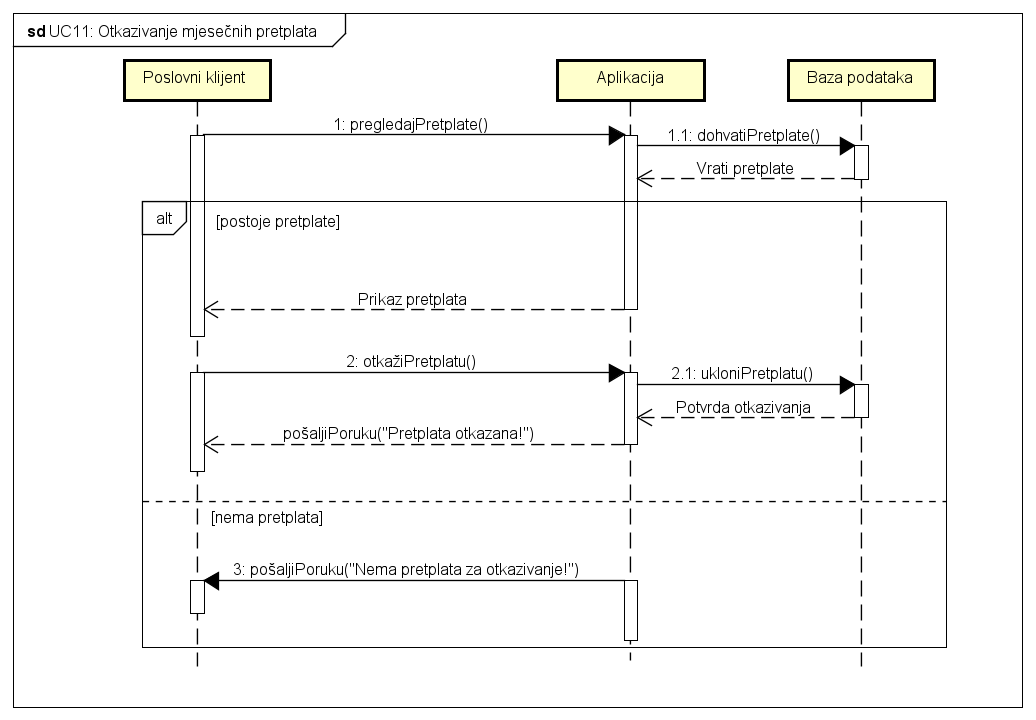
\includegraphics[scale=0.6]{dijagrami/sekv_uc11.PNG} 
				\centering
				\caption{Sekvencijski dijagram za UC11 - Otkazivanje mjesečnih pretplata}
				\label{fig:sekv_uc11}%label mora biti drugaciji za svaku sliku
			\end{figure}
		
			\textbf{UC14: Naručivanje usluga}\\
			\noindent \normalsize{Klijent odabire pregled košarice. Ako košarica nije prazna, prikazuje se njezin sadržaj i tada klijent može potvrditi narudžbu. U suprotnom, dolazi mu poruka da je košarica prazna (nema opciju  potvrditi narudžbu.)} \\
			\begin{figure}[H]
				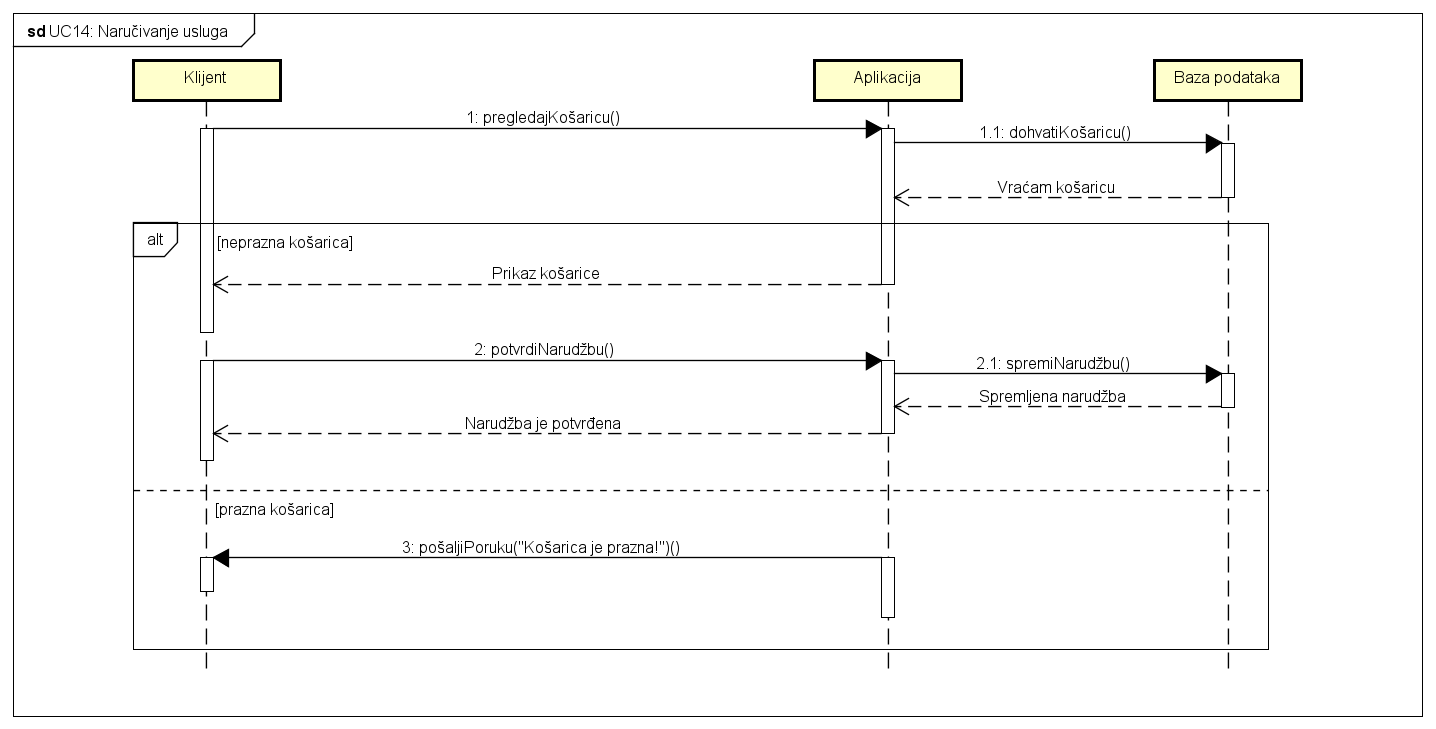
\includegraphics[scale=0.5]{dijagrami/sekv_uc14.PNG} 
				\centering
				\caption{Sekvencijski dijagram za UC14 - Naručivanje usluga}
				\label{fig:sekv_uc14}%label mora biti drugaciji za svaku sliku
			\end{figure}
		
			\textbf{UC25: Otkazivanje mjesečne pretplate poslovnih klijenata}\\
			\noindent \normalsize{Administrator odabire prikaz svih pretplata postojećih poslovnih klijenata. Među njima odabire neku pretplatu nekog od njih i otkazuje ju. Time se ta pretplata za tog klijenta briše.} \\
			\begin{figure}[H]
				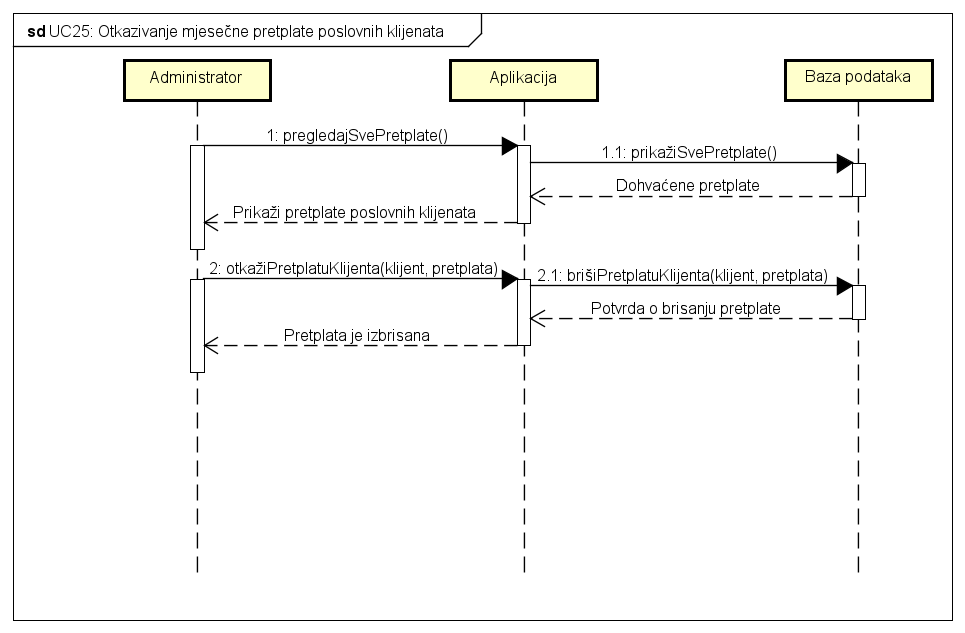
\includegraphics[scale=0.6]{dijagrami/sekv_uc25.PNG} 
				\centering
				\caption{Sekvencijski dijagram za UC25 - Otkazivanje mjesečne pretplate poslovnih klijenata}
				\label{fig:sekv_uc25}%label mora biti drugaciji za svaku sliku
			\end{figure}
				\eject
	
		\section{Ostali zahtjevi}
		
			%\textbf{\textit{dio 1. revizije}}\\
		 
			% \textit{Nefunkcionalni zahtjevi i zahtjevi domene primjene dopunjuju funkcionalne zahtjeve. Oni opisuju \textbf{kako se sustav treba ponašati} i koja \textbf{ograničenja} treba poštivati (performanse, korisničko iskustvo, pouzdanost, standardi kvalitete, sigurnost...). Primjeri takvih zahtjeva u Vašem projektu mogu biti: podržani jezici korisničkog sučelja, vrijeme odziva, najveći mogući podržani broj korisnika, podržane web/mobilne platforme, razina zaštite (protokoli komunikacije, kriptiranje...)... Svaki takav zahtjev potrebno je navesti u jednoj ili dvije rečenice.}
			
			\begin{packed_enum}
				
			
				\item Pristupanje bazi podataka ne smije trajati predugo (više od nekoliko sekundi)
				\item Sustav treba omogućiti rad više korisnika u stvarnom vremenu
				\item Nadogradnje sustava ne smiju narušavati funkcionalnosti sustava koje već postoje
				\item Sustav će biti implementiran u obliku aplikacije koristeći objektno-orijentirane jezike
				\item Aplikacija treba biti jednostavna i intuitivna za korištenje
				\item Kao valutu aplikacija koristi hrvatsku kunu - HRK 
				
				%% sadržaj će biti dodan još i prije 2. rev
				
				
			\end{packed_enum}
			 
			 
			 
	